%%%%%%%%%%%%%%%%%%%%%%%%%%%%%%%%%%%%%%%%%%%%%%%%%%%%%%%%%%%%%%%%%%%%%%%%%%%%%%%%
\chapter{System architecture and Methods}\label{ch:architecture}
%%%%%%%%%%%%%%%%%%%%%%%%%%%%%%%%%%%%%%%%%%%%%%%%%%%%%%%%%%%%%%%%%%%%%%%%%%%%%%%%


In this chapter, we will present our tool which aims to fill the gaps addressed in the chapter ~\ref{ch:introduction}. We call it \textit{SIMITAR}, an acronym for \textit{SnIffing, ModellIng and TrAffic geneRation}.  This acronym summarizes its operation. SIMITAR is a traffic generator able to learn features of a real traffic automatically, and reproduce a synthetic traffic similar to the original. It records a model for the traffic in an XML file we call \textit{compact trace descriptor} (CTD file). As input-data SIMITAR can use \textit{pcap} files or real-time captures.  


\begin{figure*}[ht!]
	\centering
	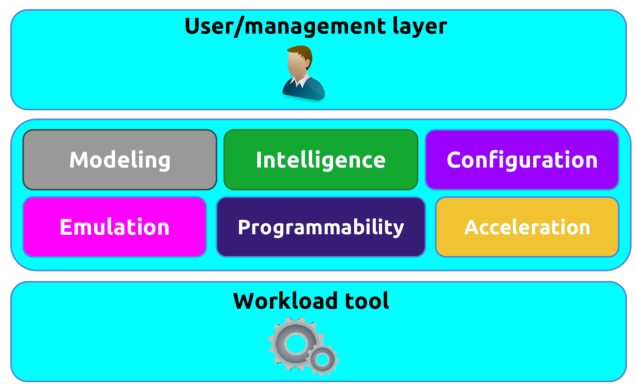
\includegraphics[height=2.4in]{figures/ch1/layer-diagram}
	\caption{ Architecture conceptual idea: a toll to automatize many tasks on traffic modelling and generation.}
	\label{fig:layer-diagram}
\end{figure*}

On the figure ~\ref{fig:layer-diagram} we abstract our concepts we stated in a layer diagram model. Or tool must work as an interface for the user automatizing traffic modeling, configuration, and emulation and offer services of intelligence and traffic generation programmability. In the figure, we also include packet-acceleration\footnote{Packet acceleration is a concept introduced by DPDK\cite{web-dpdk}, which means kernel by-pass. Packet acceleration optimizes the packet processing, and therefore traffic generation, enabling higher throughput rates.}, however, in the current version, this feature is not implemented, but how to do it is discussed in the section of future works in the chapter ~\ref{ch:conclusion}. To avoid confusions, we will refer to the underlying workload tool as packet generator engine/tool, and for SIMITAR as a traffic generator. Even if this packet generator may be a traffic generator itself (such as Iperf), on SIMITAR, its operates just on the packet-level, as we explain in the chapter ~\ref{ch:literature-review}, and our tool is a multi-layer traffic generator tool.


Our primary goal is to offer simple configuration, with \textbf{realism}, at a reasonable speed. The intermediate layer of the figure ~\ref{fig:layer-diagram} summarize, the goal of the project in an illustrative way. Instead of storing a huge file \textit{pcap} with a size of many \textit{gigas}, we create a light-weight set of models and parameters that describe this same trace. We are also introducing the concept of \textbf{programmability}. Since the \textit{compact trace descriptor},  is an XML file, the user may create his custom traffic in a platform agnostic way creating his own CTD file. So the will be able to create multi-flow Ethernet workload not having to create many scripts for each tool or reading its documentation. A single description of the traffic will fit any supported packet generator. Using a component methodology, we decouple the packet generation, from the data collection and parameterization process. We developt it using the design pattern factory to make the extension easy for any packet generator engine. 


We abstract its whole operation cycle in the figure ~\ref{fig:cycle-of-operation}. Our tool, from live captures or \textit{pcap} file collects raw data from Ethernet traffic. It then breaks these data into different flows and uses this data to generate a set of parameters for our traffic model, using a set of algorithms. Finally, SIMITAR provides these parameters to a packet generator engine and controls its packets injection.

% cycle of operation
\begin{figure*}[ht!]
        \centering
        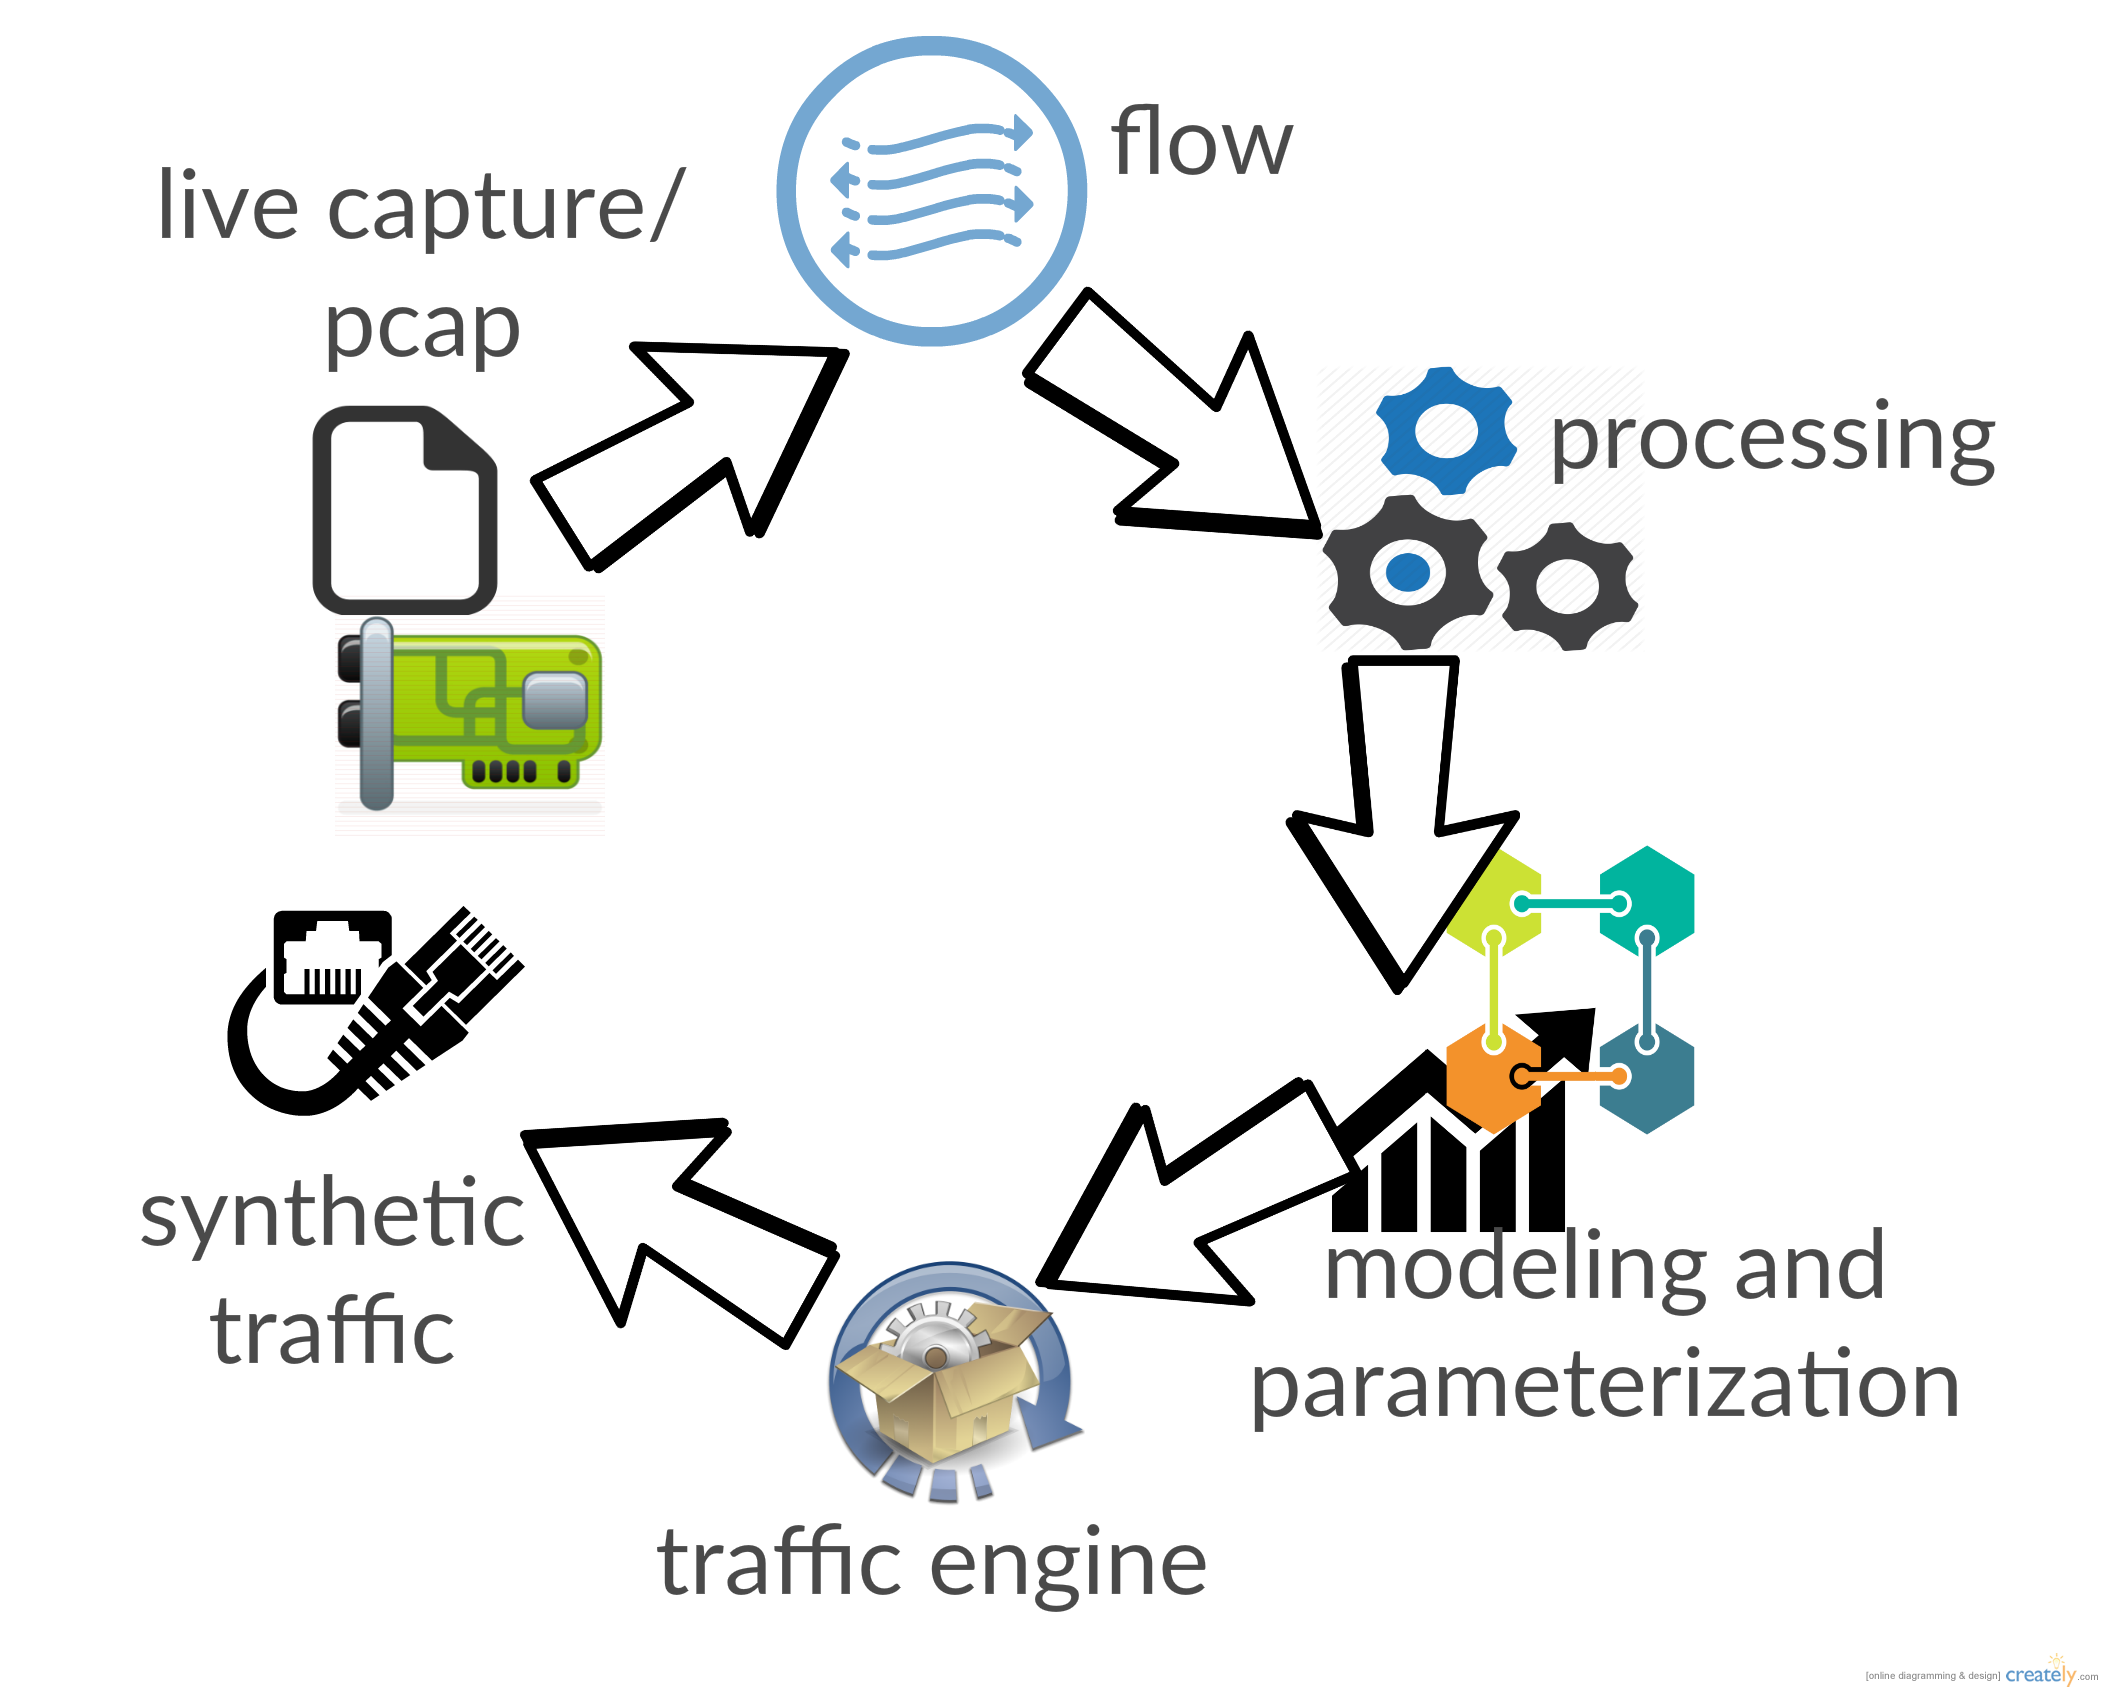
\includegraphics[height=3.0in]{figures/ch3/digram-project-cycle}
        \caption{This figure represents an operation cycle of SIMITAR, emphasizing each main step: sniffing, flow classification, data storing, data processing and fitting, model parameterization,  and synthetic traffic generation.}
    \label{fig:cycle-of-operation}
\end{figure*}


%%%%%%%%%%%%%%%%%%%%%%%%%%%%%%%%%%%%%%%%%%%%%%%%%%%%%%%%%%%%%%%%%%%%%%%%%%%%%%%%
\section{SIMITAR Architecture}


To meet the requirements presented in the chapter ~\ref{ch:introduction}, we will define our solution, and how it works. SIMITAR architecture is presented in the figure~\ref{fig:architecture}. It is composed of four components: a \textit{Sniffer}, a \textit{SQLite database}, a \textit{TraceAnalyzer}, a \textit{FlowGenerator};  and a \textit{Network Traffic Generator}, as subsystem. We describe each part below.

% component diagram and module design
\begin{figure*}[ht!]
        \centering
        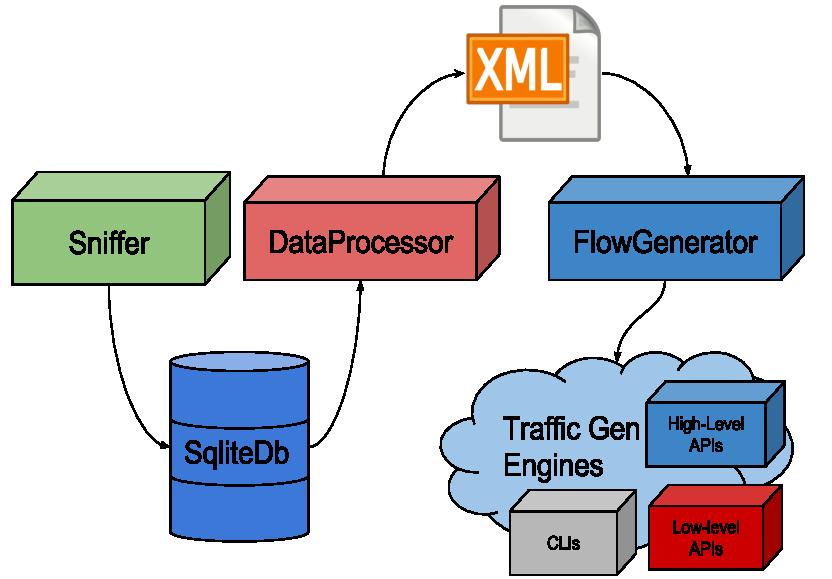
\includegraphics[height=2.7in]{figures/ch3/architecture-diagram}
        \caption{Architecture of SIMITAR}
    \label{fig:architecture}
\end{figure*}


%%%%%%%%%%%%%%%%%%%%%%%%%%%%%%%%%%%%%%%%%%%%%%%%%%%%%%%%%%%%%%%%%%%%%%%%%%%%%%%%
\subsection{Sniffer}



This component collects network traffic data and classifies it into flows, storing stores in an SQLite database. It defines each flow by the same criteria used by SDN switches\cite{sdn-survey},  through header fields matches. It uses:

\begin{itemize}
\item Link Protocol
\item Network Protocol
\item Network Source and Destination Address
\item Transport Protocol
\item Transport Source and Destination Port
\end{itemize}

\begin{figure*}[ht!]
        \centering
        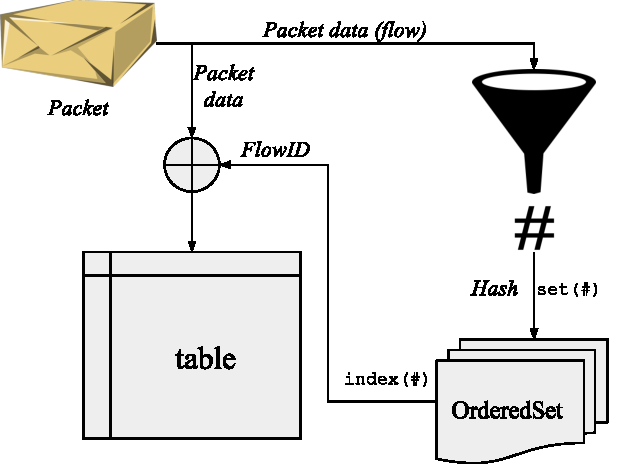
\includegraphics[height=2.5in]{figures/ch3/sniffer-classifier}
        \caption{SIMITAR's sniffer hash-based flow classification}
    \label{fig:sniffer}
\end{figure*}


We implemented the first version of this component in Shell Script (Bash).  Tsahrk\footnote{\href{https://www.wireshark.org/docs/man-pages/tshark.html}{https://www.wireshark.org/docs/man-pages/tshark.html}} was used to extract header fields, and Awk to match the flows, and Sed/Awk to create the SQLite queries. This version was too slow to operate in real time on Ethernet interfaces. On the other hand, this approach was fast to implement and enable the implementation of the other components. The second and current version was made using Python. This version used Pyshark \footnote{\href{https://pypi.python.org/pypi/pyshark}{https://pypi.python.org/pypi/pyshark}} as sniffer library.  


It has a data structure we developed called \textit{OrderedSet}. A set is a list of elements with no repetition but does not keep track of the insertion order. Our OrderedSet does. Also, it makes use of a  64 bits hash function of the family FNV\footnote{The collision probability of a good 64 bits hash function in a table with 10000 items is about of $2.71e-12$.}. The listed header fields are inputs for a hash function, and its value is set on the ordered set which returns its order (index on the \textit{OrderedSet}). The index value is chosen as a packet flowID.  


%c++ http://ideone.com/F0V42m
As future improvements for this component, we propose a more efficient implementation in C++ and data visualization for the collected data. In that way, we may optimize the packet processing. We discuss this in deeper details in the chapter~\ref{ch:conclusion}.


%%%%%%%%%%%%%%%%%%%%%%%%%%%%%%%%%%%%%%%%%%%%%%%%%%%%%%%%%%%%%%%%%%%%%%%%%%%%%%%%
\subsection{SQLite database}

\begin{figure*}[ht!]
        \centering
        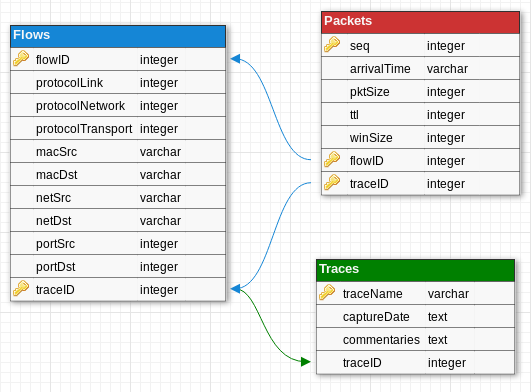
\includegraphics[height=3.0in]{figures/ch3/database-relational-model}
        \caption{SIMITAR's SQLite database relational model}
    \label{fig:simitar-database}
\end{figure*}

% ok1

The database stores the collected raw data from the traces for further analysis. The \textit{Sniffer} and the \textit{TraceAnalyzer} components uses the database.  We choose an SQLite database, because according to its specifications\footnote{\href{https://www.sqlite.org/whentouse.html}{https://www.sqlite.org/whentouse.html}}, it fits well our purposes. It is simple and well-suitable for an amount of data smaller than terabytes. In the figure ~\ref{fig:simitar-database} we present the relational model of our database, which stores a set of features extracted from packets, along with the flowID calculated by the sniffer component. 


%%%%%%%%%%%%%%%%%%%%%%%%%%%%%%%%%%%%%%%%%%%%%%%%%%%%%%%%%%%%%%%%%%%%%%%%%%%%%%%%
\subsection{Trace Analyzer}


This module is the core of our project. It creates a trace model via the analysis of the collected data. We define here a Compact Trace Descriptor (CTD) as a human and machine-readable file, which describes a traffic trace through a set of flows, each of them represented by a set of parameters, such as header information and analytical models.  The Trace Analyze has the task to learn these features from raw traces data (stored in the SQLite database) and generate an XML file.  In the figure~\ref{fig:CTD-diagram} we show a directory diagram of a CDT file. It has many of many flow fields, and each one contains each parameter estimated. Now we will describe how we construct it. 


\begin{figure}
\centering
\subfloat[]{
  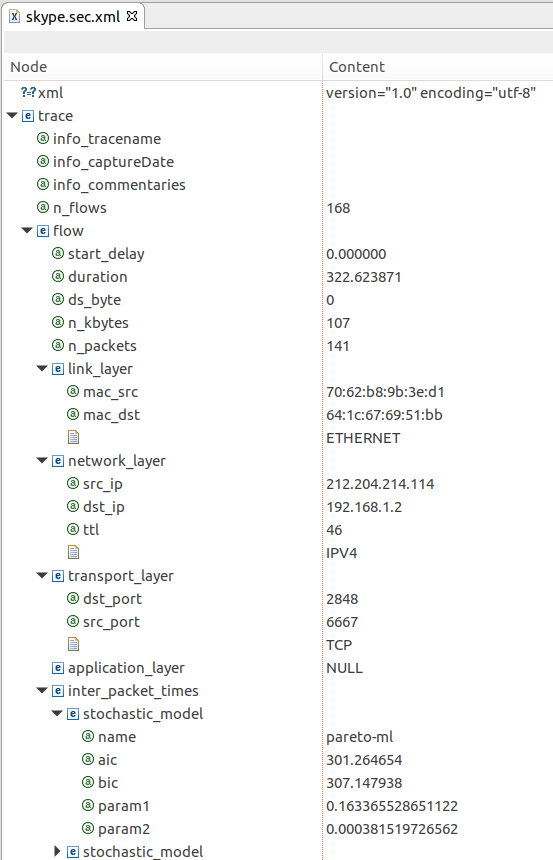
\includegraphics[height=4.in]{figures/ch3/cdt1}
}
\subfloat[]{
  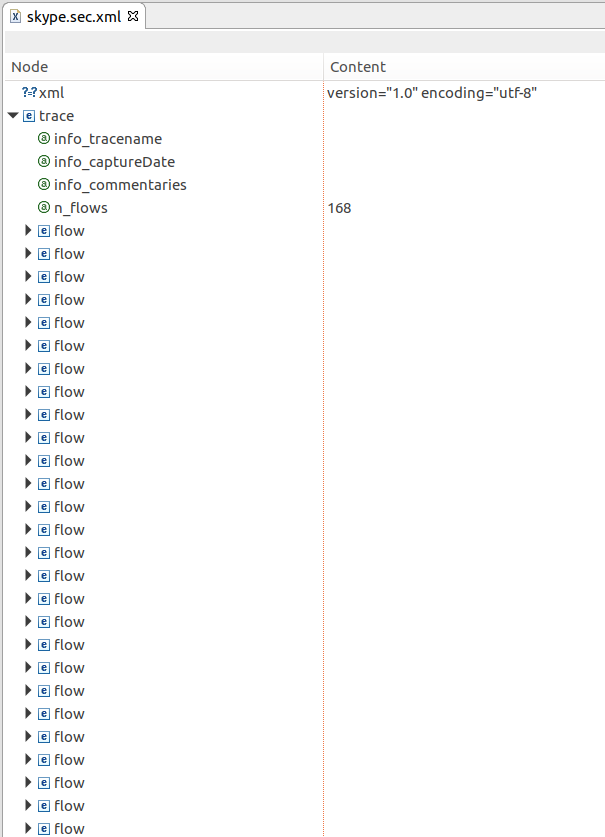
\includegraphics[height=4.in]{figures/ch3/cdt2}
}
\caption{Directory diagram of the schema of a Compact Trace Descriptor (CDT) file. On the left, we present a dissected flow, and on the right a set of flows.}
\label{fig:CTD-diagram}
\end{figure}


%%%%%%%%%%%%%%%%%%%%%%%%%%%%%%%%%%%%%%%%%%%%%%%%%%%%%%%%%%%%%%%%%%%%%%%%%%%%%%%%
\subsubsection{Flow features}


Some unique per-flow features are directly measured from the data. They are:  

\begin{itemize}
\item Flow-level properties like duration of flow, start delay, number of packets per flow, number of KBytes per flow; 
\item Header fields, like protocols, QoS fields, ports, and addresses.
\end{itemize}

Each one of these parameters is unique per flow. Other features like PSD (packet size distribution) e IPT (Inter-packet time), have a more complex behavior.  To represent these characteristics, we will use sets of stochastic-based models.  


\subsubsection{Inter Packet Times}

\begin{figure*}[ht!]
    \centering
    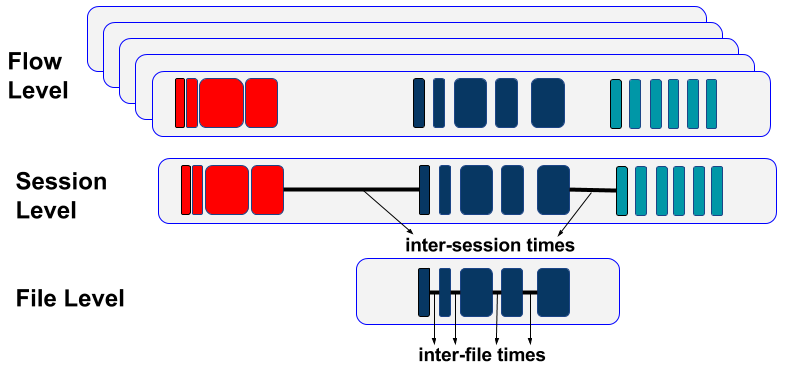
\includegraphics[height=2.0in]{figures/ch3/modified-harpoon-model}
    \caption{The schema of the modified version of the Harpoon algorithm we adopt on SCIMITAR.}
    \label{fig:modified-harpoon-model}
\end{figure*}


To represent inter-packet times, we adopt a simplified version of the Harpoon's traffic model. A deep explanation of the original model can be found at \cite{harpoon-paper} and \cite{harpoon-validation}. Here, we will explain our simplified version, which is illustrated at figure~\ref{fig:modified-harpoon-model}. Harpoon uses a definition of each level, based on the measurement of SYN and ACK TCP flags. It uses TCP flags (SYN) to classify packets in different levels, named their file, session, and user level. We choose to estimate these values, based on inter-packet times only. The distinction is made based on the time delay between packets.


In our algorithm simplified version, we define three different layers of data transference to model and control: file, session, and flow. For SIMITAR, a file is just a sequence of consecutive packets transmitted continuously, without large interruption of traffic. It can be, for example, packets sent downloading a file, packets from a  UDP  connection or a single ICMP echo packet. The session-layer refers to a sequence of multiple files transmitted between a source and a destination, belonging to the same flow.  The flow level refers to the conjunct of flows, as classified by the Sniffer.  Now, we explain SIMITAR operation on each layer. 


In the \textbf{flow layer} the \textit{TraceAnalyzer} loads the flow arrival times from the database and calculates the inter-packet times within the flow context. At the \textbf{session layer}, we use a deterministic approach for evaluating file transference time and times between files: ON/OFF times sequence of packet trains. We choose a deterministic model because in this way we can express diurnal behavior\cite{harpoon-paper}.  We develop an algorithm called \textit{calcOnOff} responsible for estimating these times. It also determines the number of packets and bytes transferred by each file. Since the ON times will serve as input for actual traffic generators, we defined a minimum acceptable time for on periods equals to 100 ms. ON times can be arbitrary smalls, and they could be incompatible with acceptable ON periods for traffic generators. Also in the case of just one packet, the ON time would be zero. So setting a minimum acceptable time to solve these issues. The OFF times, on the other hand, are defined by the constant \texttt{session\_cut\_time} \footnote{In the code it is called \texttt{DataProcessor::m\_session\_cut\_time} }. If the time between two packets of the same flow is larger than \texttt{session\_cut\_time}, we consider them belonging to a different file, so this time is a session OFF time. In this case, we use the same value of the constant \textit{Request and Response timeout} of Swing\cite{swing-paper} for the \texttt{session\_cut\_time}: 30 seconds. The control of ON/OFF periods in the traffic generation is made by the \textit{Flow Generator} component \footnote{This control is made by the class \texttt{NetworkFlow}}.


In the \textbf{file layer}, we model the inter-packet times at the file level. To estimate inter-packet times within files, we select all inter-packet times smaller than \texttt{session\_cut\_time}\footnote{In the code it is called\texttt{DataProcessor::m\_session\_cut\_time} }. All files within the same flow are considered to follow the same model. We delegate the control of the inter-packet times to the underlying packet generator engine. We ordered them, from the best to the worst. Currently, we are using eight different stochastic functions parameterizations. They are Weibull(linear regression), Normal(mean/standard deviation calculation), Exponential(mean and linear regression estimation), Pareto(linear regression and maximum likelihood), Cauchy(linear regression) and Constant(mean calculation). From those, Weibull, Pareto, and Cauchy are heavy-tailed functions, and therefore self-similar processes. But if the flow has less than 30 packets, just the constant model is evaluated. It is because numerical methods gave poor results if the data sample used is small. We sort these models according to the Akaike Information Criterion (AIC) as default\cite{sourcesonoff-paper}\cite{bic-aic-comparision}. We will enter into deeper details on this methodology on the chapter ~\ref{ch:modeling-evaluation}. The methodology of selection is presented in the figure~\ref{fig:model-parameterization}, and all constants and modes of operation can be changed by command line options.


\begin{figure*}[ht!]
    \centering
    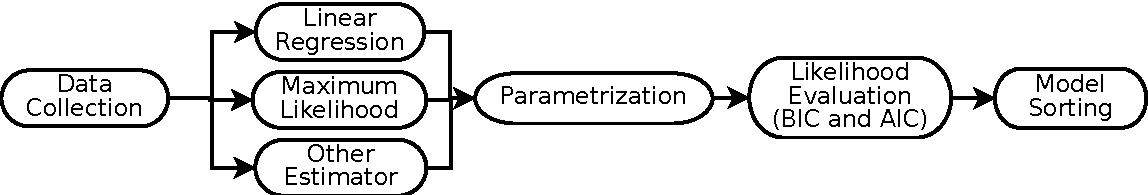
\includegraphics[height=0.9in]{figures/ch3/simitar-parametrization}
    \caption{Diagram of parameterization and model selection for inter-packet times and inter-file times.}
    \label{fig:model-parameterization}
\end{figure*}


\subsubsection{Packet Sizes}



Our approach for the packet size is much simpler. Since the majority of packet size distribution found on real measurements are bi-modal \cite{packet-distribution-model}\cite{sourcesonoff-paper}\cite{udp-flows-model}, we first sort all packet sizes of flow in two modes. We define a packet size mode cut value of 750 bytes, same value adopted by \cite{udp-flows-model}. 


We know how much packets each mode has, and then we fit a model for it. We use three stochastic models: constant, exponential and normal. Since self-similarity does not make sense for packet-sizes, we prefer to use just the simpler models. When there is no packet for a model, we set a flag NO\_MODEL, and when there is just a single packet we just use the constant model. Then calculate the BIC and AIC for each, but we decide to set the constant model as the first.

As is possible to see in many works \cite{packet-distribution-model} \cite{udp-flows-model}, since the standard deviation of each mode tends to be small, constant fittings use to give good approximations. Also, it is computationally cheaper for the traffic generated than the other models, since no calculation is a need for each packet sent. Since both AIC and BIC criteria always will select the constant model as the worst, we decide to ignore this.


\subsubsection{Compact Trace Descriptor}
%<<<<<<<<<<<<<<<<<<<<<<<<<<<<<<<<<<<<<<<<<<<<<<<<<<<<<<<<<<<<<<<<<

%2nd-review
An example of the final result of all the methods is presented in the XML code down below. It illustrates a flow of a \textit{Compact Trace Descriptor}(CDT) file. The traffic models for inter-packet times are grouped by the tag \texttt{inter\_packet\_times}, and the packet trains by the tag \texttt{session\_times}. All the times are in seconds, and "\texttt{inf}" represents infinity. The protocol of each layer is stored as data by each tag.

\begin{minted}[frame=single,
               framesep=3mm,
               linenos=true,
               xleftmargin=21pt,
               tabsize=4,
               fontsize=\scriptsize, 
               breaklines=true]{xml}
               
	<flow start_delay="0.144400" duration="317.744333" ds_byte="0" n_kbytes="40" n_packets="344">
		<link_layer mac_src="64:1c:67:69:51:bb" mac_dst="70:62:b8:9b:3e:d1">ETHERNET</link_layer>
		<network_layer src_ip="192.168.1.1" dst_ip="192.168.1.2" ttl="64">IPV4</network_layer>
		<transport_layer dst_port="2128" src_port="53">UDP</transport_layer>
		<application_layer>DNS</application_layer>
		<inter_packet_times>
			<stochastic_model name="pareto-ml" aic="-1165.310696" bic="-1157.646931" param1="0.405085202535192" param2="0.002272655895996"/>
			<stochastic_model name="pareto-lr" aic="-454.049749" bic="-446.385984" param1="0.061065000000000" param2="0.002272655895996"/>
			<stochastic_model name="weibull" aic="-246.882037" bic="-239.218273" param1="0.120355000000000" param2="0.001629000000000"/>
			<stochastic_model name="exponential-me" aic="486.370061" bic="494.033826" param1="1.340057495455104" param2="0.000000000000000"/>
			<stochastic_model name="normal" aic="1629.370900" bic="1637.034665" param1="0.746236637899171" param2="2.626808289821357"/>
			<stochastic_model name="exponential-lr" aic="3166.816047" bic="3174.479812" param1="0.009752000000000" param2="0.000000000000000"/>
			<stochastic_model name="cauchy" aic="31737.418442" bic="31745.082207" param1="0.000000000000194" param2="-3152.827055696396656"/>
			<stochastic_model name="constant" aic="inf" bic="inf" param1="0.746236637899171" param2="0.000000000000000"/>
		</inter_packet_times>
		<session_times on_times="29.22199798,73.40390396,151.84077454" off_times="30.85738373,32.42027283" n_packets="19,103,222" n_bytes="2272,12399,26689"/>
		<packet_sizes n_packets="344" n_kbytes="40">
			<ps_mode1 n_packets="344" n_kbytes="40">
				<stochastic_model name="constant" aic="inf" bic="inf" param1="120.232558" param2="0.000000"/>
				<stochastic_model name="normal" aic="2926.106952" bic="2933.788235" param1="120.232558" param2="16.941453"/>
				<stochastic_model name="exponential-me" aic="3987.126362" bic="3994.807645" param1="0.008317" param2="0.000000"/>
			</ps_mode1>
			<ps_mode2 n_packets="0" n_kbytes="0">
				<stochastic_model name="no-model-selected" aic="inf" bic="inf" param1="0.000000" param2="0.000000"/>
			</ps_mode2>
		</packet_sizes>
	</flow>
	
\end{minted}

%2nd-review
%The current version of our tool, do not intrinsically supports responsiveness. The underlying traffic generator API can support it (such as Seagull\cite{web-seagull}), but we do not generate any mathematical model for this purpose, and this may also stand as a future work we discuss on chapter ~\ref{ch:conclusion}. 


%%%%%%%%%%%%%%%%%%%%%%%%%%%%%%%%%%%%%%%%%%%%%%%%%%%%%%%%%%%%%%%%%%%%%%%%%%%%%%%%
\subsection{Flow Generator}

\begin{figure*}[ht!]
	\centering
	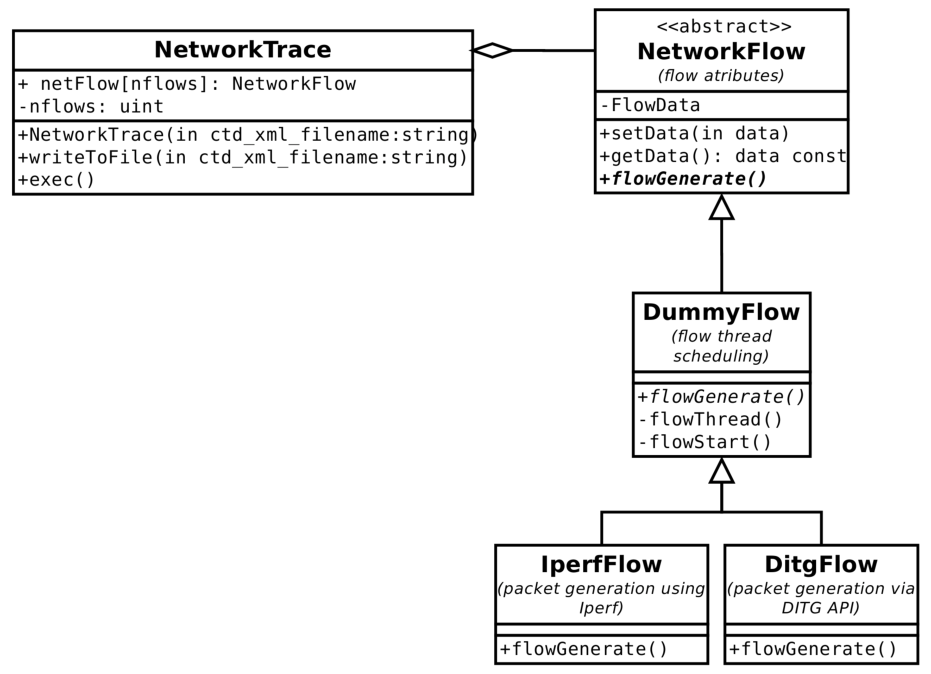
\includegraphics[height=3.0in]{figures/ch3/trace-flow}
	\caption{Class hierarchy of NetworkTrace and NetworkFlow, which enables the abstraction of the traffic generation model of the packet generation engine.}
	\label{fig:network-trace-flow-class-diagram}
\end{figure*}

\begin{figure*}[ht!]
    \centering
    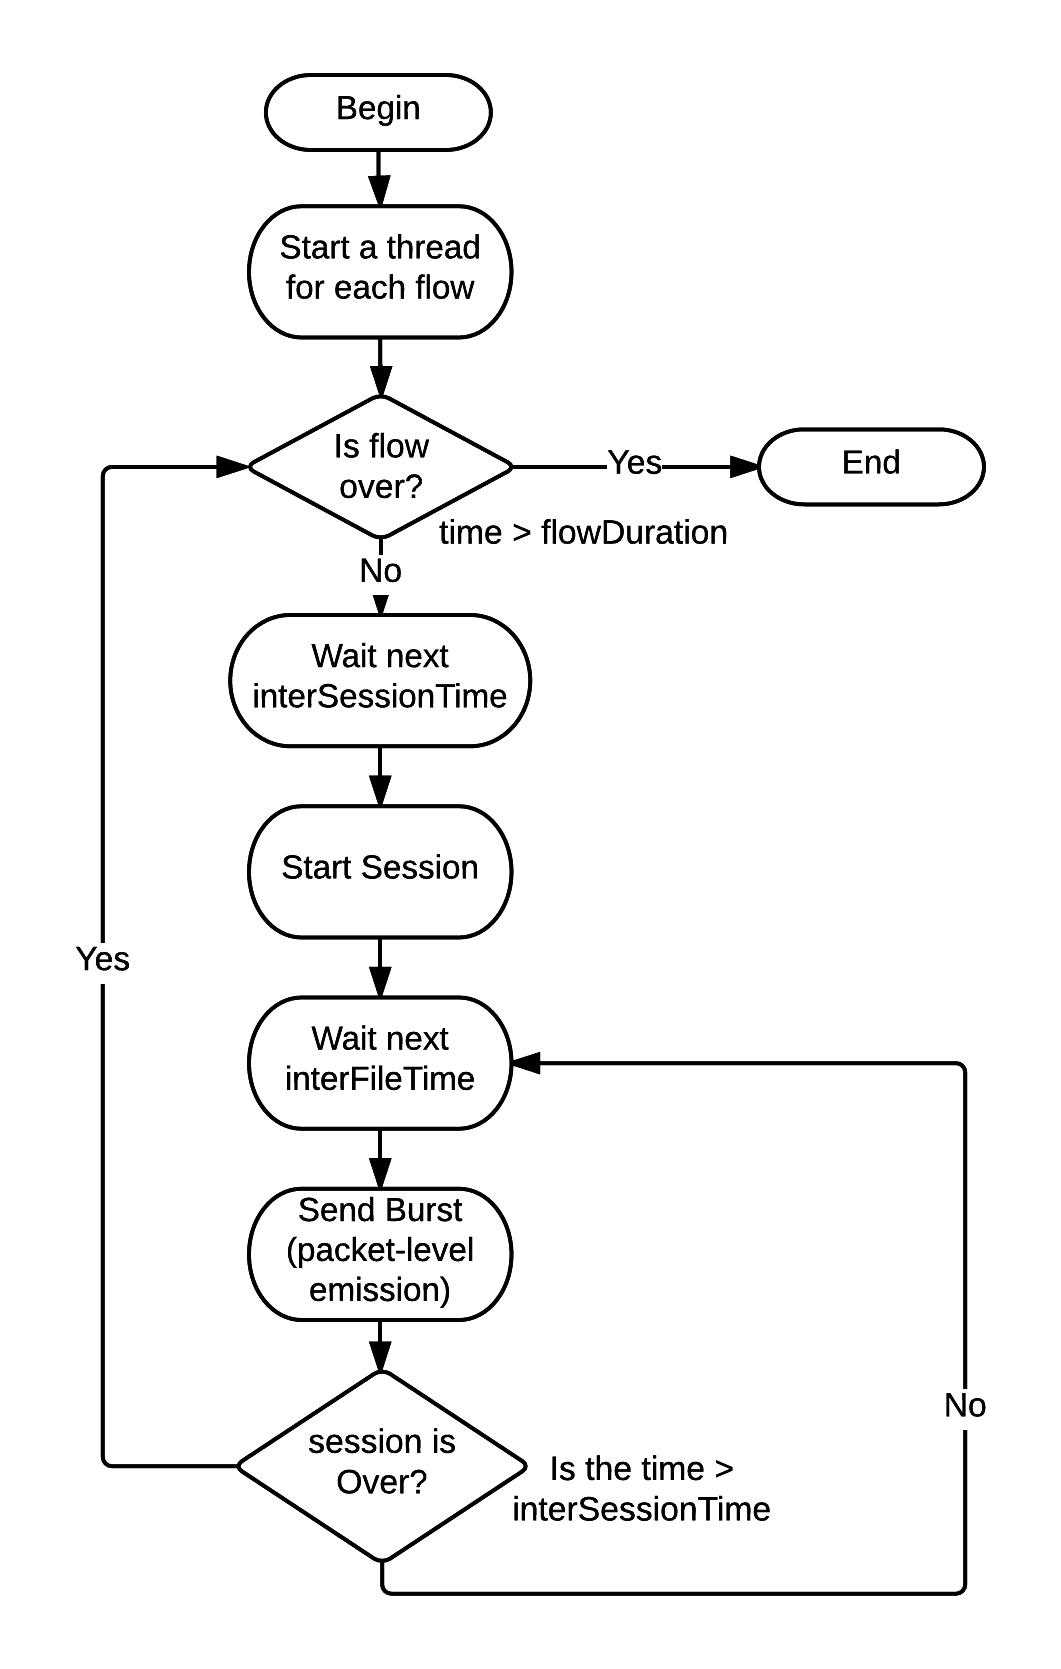
\includegraphics[height=4.5in]{figures/ch3/alg-simplified-harpoon}
    \caption{Simplified-harpoon emission algorithm}
    \label{fig:alg-simplified-harpoon}
\end{figure*}


\begin{figure*}[ht!]
	\centering
	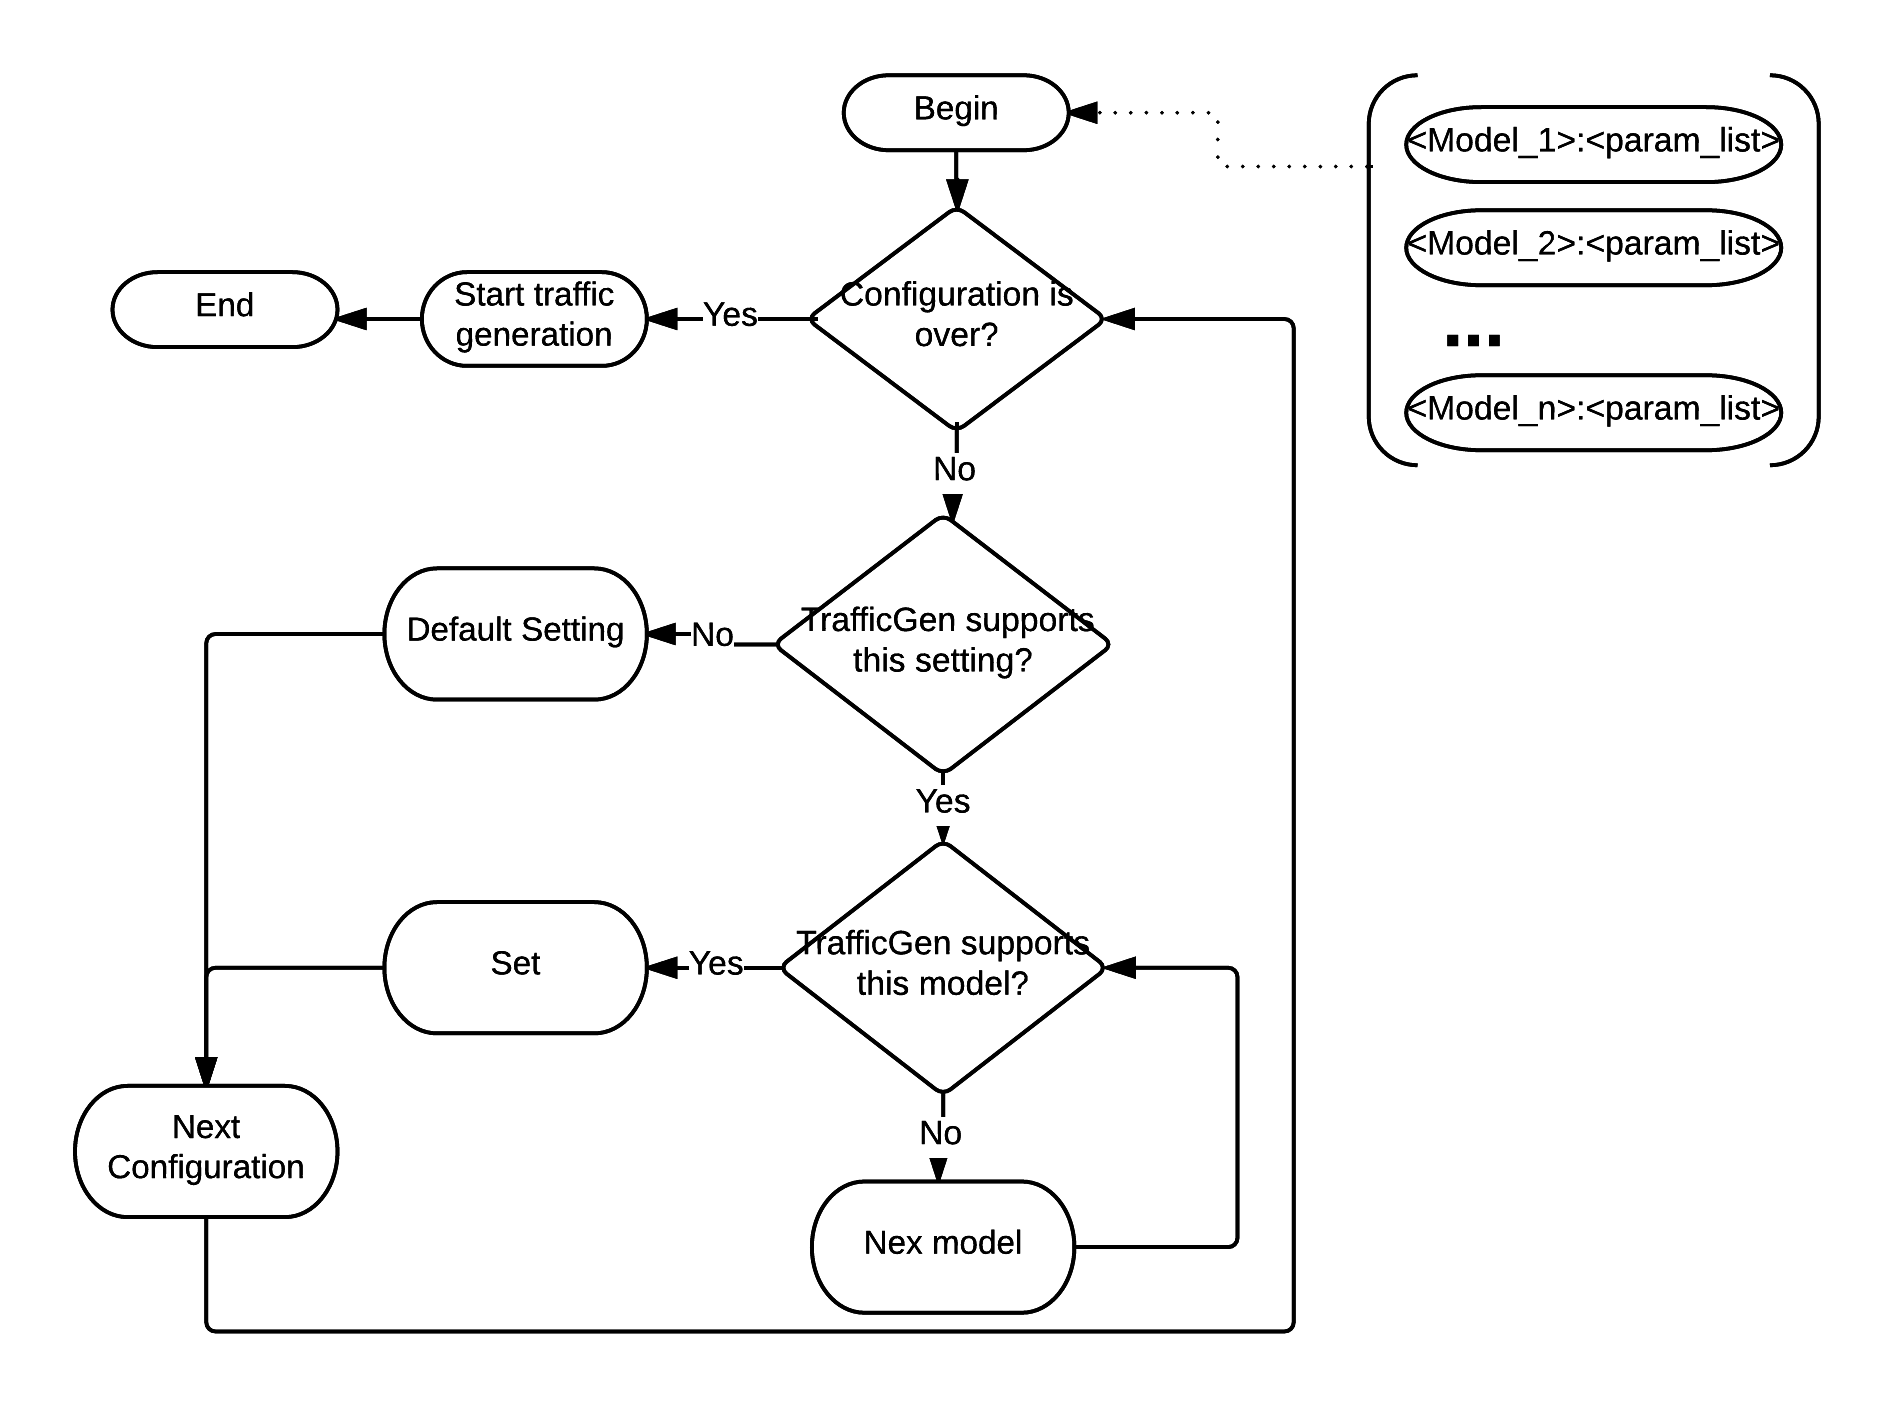
\includegraphics[height=4.0in]{figures/ch3/alg-traffic-engine-config}
	\caption{Packet engine configuration method}
	\label{fig:alg-traffic-engine-config}
\end{figure*}


The Flow Generator handles the data on the \textit{Compact Trace Descriptor} file, and use to retrieve parameters for traffic generation. It crafts and controls each flow in a separated thread. We already implemented this component using Iperf and Libtins(C++ API) as packet generators. It must follow the class hierarcy as presented in the figure ~\ref{fig:network-trace-flow-class-diagram}.  This component was designed using the design pattern Factory, to simplify its expansion and support\footnote{If the user wants to introduce support for a new packet generator engine, he just has to expand the class \texttt{DummyFlow}, creating a new derived class (figure ~\ref{fig:network-trace-flow-class-diagram} ). On our current implementation we already have implemented \texttt{IperfFlow} and \texttt{TinsFlow}, and \texttt{DitgFlow} is under validation process. This new class has the requirement of not have any new attribute. The support for this new class must be given on the factory class \texttt{NetworkFlowFactory}. For closed loop packet-crafters (that means, tools which must establish a connection between the source and the destination), two methods must be implemented: \texttt{flowGenerate()} and \texttt{server()}. \texttt{flowGenerate()} is responsible for sending a \textit{file}, as defined on de figure~\ref{fig:modified-harpoon-model}, and \texttt{server()} to receive $n$ files. Open loop packet-crafters, such as we implemented using Libtins (just sent the packets, do not establishes a connection), the server do not need to be implemented.}. 



This component itself is a multi-layer workload generator according to the typing introduced on chapter ~\ref{ch:literature-review} \footnote{Since it works both at packet and flow level, but do not work at application level.}. At the flow-level, SIMITAR controls each flow using the algorithm at figure~\ref{fig:alg-simplified-harpoon}. This algorithm handles our model defined at the figure ~\ref{fig:modified-harpoon-model}. This procedure is independent of the underlying packet crafting tool used. It starts a \textit{thread} for each flow in the \textit{Compact Trace Descriptor}, then the thread sleeps for \texttt{start\_delay} seconds. This is the arrival time of the first flow packet. Passed this time, it then calls the underlying packet generator tool(defined as command line argument), and pass to it the flowID, file ON time, number of packets and number of bytes to be sent (file size), and network interface. Then it sleeps the next session OFF time. When the list of ON/OFF times from the flow is over, the thread ends. 


At the packet level, SIMITAR configures the packet-generator tool to send a \textit{file}, as defined in the figure ~\ref{fig:modified-harpoon-model}. This method must use the available parameters, attributes and \textit{getters} to configure and generate a thread-safe traffic using the method \texttt{flowGenerate()}. The \textit{file} configuration must follow the in the figure ~\ref{fig:alg-traffic-engine-config}.  Down below we present a simple code of how the D-ITG API can be used to generate packet-level traffic. A more complex configuration is possible, but it serves to illustrate the procedure. We call this concept \textit{Flow Generation Programming}.  Its API documentation is available at on D-ITG website \footnote{\href{http://www.grid.unina.it/software/ITG/manual/index.html\#SECTION00047000000000000000}{http://www.grid.unina.it/software/ITG/manual/index.html\#SECTION00047000000000000000}}. 


\begin{minted}[frame=single,
               framesep=3mm,
               linenos=true,
               xleftmargin=21pt,
               tabsize=4,
               fontsize=\scriptsize, 
               breaklines=true]{c++}


// This implementation is just a simplified version to illustrate the procedure.
void DitgFlow::flowGenerate(const counter& flowId, const time_sec& onTime, const uint& npackets, const uint& nbytes,  const string& netInterface)
{
	// create command to generate the traffic
	std::string strCommand;
	std::string localhost = getNetworkSrcAddr(); 
	strCommand += " -t " + std::to_string(onTime); 
	strCommand += " -k " + std::to_string(nbytes / 1024);
	strCommand += " -a " + getNetworkDstAddr();
	
	// configure protocol
	if (this->getTransportProtocol() == PROTOCOL__TCP)
		strCommand += " -T TCP -D ";
	else if (this->getTransportProtocol() == PROTOCOL__UDP)
		strCommand += " -T UDP ";
	else if (this->getTransportProtocol() == PROTOCOL__ICMP)
		strCommand += " -T ICMP ";
		
	//configure inter-packet time model, just Weibull or Constant
	StochasticModelFit idtModel;
	for(uint i = 0;;i++)
	{	
		idtModel = this->getInterDepertureTimeModel(i);
		if(idtModel.modelName() == WEIBULL)
		{
			strCommand += " -W " + std::to_string(idtModel.param1()) + " " + std::to_string(idtModel.param2());
			break;
		}
		else if ( idtModel.modelName() == CONSTANT)
		{
			strCommand += " -C " + std::to_string(nbytes/(1024*onTime));
			break;
		}
	}
	
	// it uses C strings as arguments
	// it is not blocking, so it must block until finishes
	int rc = DITGsend(localhost.c_str(), command.c_str()); // D-ITG API
    usleep(onTime*10e6); // D-ITG uses miliseconds as time unity
	if (rc != 0)
	{
		PLOG_ERROR << "DITGsend() return value was" << rc ; // our log macro for erros
		exit(EXIT_FAILURE);
	}
}
\end{minted}


%%%%%%%%%%%%%%%%%%%%%%%%%%%%%%%%%%%%%%%%%%%%%%%%%%%%%%%%%%%%%%%%%%%%%%%%%%%%%%%%
\subsection{Network Packet Generator}


A network packet generator is a tool or lybrary that should provide its API or script interface\footnote{In the case of a tool with a available CLI, to use it as packet generator we must use functions such as \texttt{fork()} or \texttt{popen()}. For Iperf, we used \texttt{popen()}.} for the \textit{FlowGenerator} component. With this engine, the user must be eble to send packets and controll atributes such as sending time, bandwidth, number of packets, protocols, and so on. That means, any available parameter form the compact trace descriptor.
 

%%%%%%%%%%%%%%%%%%%%%%%%%%%%%%%%%%%%%%%%%%%%%%%%%%%%%%%%%%%%%%%%%%%%%%%%%%%%%%%%
\section{Usage and Use Cases}

Each SIMITAR component works as a different application:

\begin{itemize}
	\item \textit{Sniffer}: \texttt{sniffer-cli.py};
	\item \textit{Database}: \texttt{trace.db};
	\item \textit{Trace Analyzer}: \texttt{trace-analyzer}.
	\item \textit{Flow Generator}: \texttt{simitar-gen} (the actual traffic generator).
\end{itemize}


Down below we show some usage commands of SIMITAR's components. The \texttt{sniffer-cli.py} application creates a new trace entry on the database using the command option \texttt{new}. Then the \texttt{Trace Analyzer} is able to create a \textit{compact trace descriptor} using the same trace entry. We can change the constants used by the \textit{Trace Analyzer} by command line option. As a traffic generator (\texttt{simitar-gen}), SIMITAR may work as a client or a server. Working as a server is necessary for closed-loop packet-generator engines; tools that require establishing a connection before generating the traffic, such as Iperf and D-ITG. It will just work passively. Working as a client is acting as a traffic emitter. Open loop packet-crafter tools such as \textit{libtins} does not require server operation to send the traffic. In case of closed-loop tools, the destination IP addresses must be explicitly given in the command line by the options \texttt{--dst-list-ip} or \texttt{--dst-ip}. 


\begin{minted}[frame=single,
               framesep=3mm,
               linenos=true,
               xleftmargin=21pt,
               tabsize=4,
               fontsize=\scriptsize, 
               breaklines=true]{bash}

# @ SIMITAR/, load enviroment variables
source data/config/simitar-workspace-config.sh

# @ SIMITAR/sniffer/, execute to sniff the eth0 interface, and create a trace entry called "intrig" in the database
./sniffer-cli.py new intrig live eth0

# @ SIMITAR/sniffer/, execute this command to list all traces recorded in the database
./sniffer-cli.py list

# @ SIMITAR/trace-analyzer/, execute this command to create two Compact Trace Descriptors, called intrig.ms.xml and intrig.sec.xml. The first is parameterized using milisecons, and de second, uses seconds as time unity.
./trace-analyzer --trace intrig

# @ SIMITAR/simitar-gen/, execute these commands to generate traffic using the intrig.sec.xml compact trace descriptor. It is stored at the directory "../data/xml/". 
# Libtins
./simitar-gen --tool tins --mode client --ether eth0 --xml ../data/xml/intrig.sec.xml 
# Iperf
./simitar-gen --tool iperf --mode client --ether eth0 --xml ../data/xml/intrig.sec.xml --dst-ip 10.0.0.2
./simitar-gen --tool iperf --mode server --ether eth0 --xml ../data/xml/intrig.sec.xml

\end{minted}


\begin{figure*}[ht!]
	\centering
	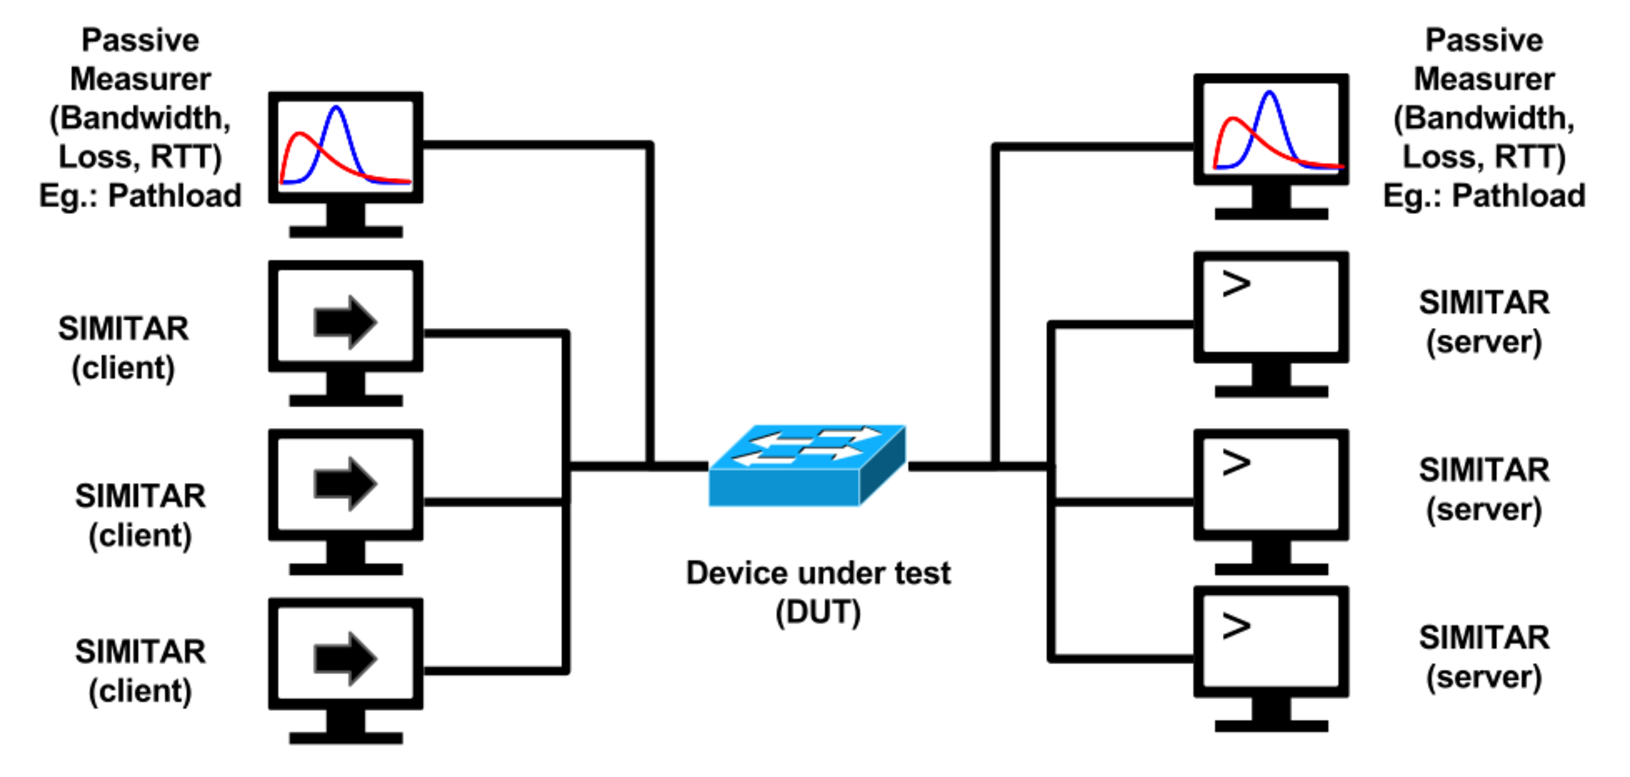
\includegraphics[height=2.4in]{figures/ch3/use-case}
	\caption{Use case example of SIMITAR}
	\label{fig:use-case}
\end{figure*}


An example of use case is presented in the figure ~\ref{fig:use-case}. A Device under test can be stressed using a combination of traffic generated by many clients and server pairs. In the case of an open-loop packet generator tool (such as in the Libtins implementation), the servers pairs are not necessary. Using passive network measures, such as Pathload and pathChirp \cite{swing-paper}, it is possible to measure statistics form the device under tests. 



